\documentclass{article}

\usepackage[utf8]{inputenc}
\usepackage[english]{babel}
 
\usepackage{multicol,caption}
%\usepackage{pgfplots}
\usepackage{graphicx}
\usepackage{footnote}
\makesavenoteenv{tabular}
\makesavenoteenv{figure}
\newenvironment{Figure}
  {\par\medskip\noindent\center\minipage{0.9\linewidth}}
  {\endminipage\par\bigskip\medskip}
  %figure inside multicols

\setlength{\oddsidemargin}{0pt}
% Marge gauche sur pages impaires
\setlength{\evensidemargin}{0pt}
% Marge gauche sur pages paires
\setlength{\textwidth}{470pt}
% Largeur de la zone de texte 
\setlength{\topmargin}{0pt}
% Pas de marge en haut
\setlength{\headheight}{13pt}
% Haut de page
\setlength{\headsep}{10pt}
% Entre le haut de page et le texte
\setlength{\footskip}{40pt}
% Bas de page + séparation
\setlength{\textheight}{630pt}
% Hauteur de la zone de texte 


\title{Heterogeneous Micro-architectural adaptation of Codelets using gem5 and CERE}
\author{Nicolas Derumigny \\
\small ENS de Lyon 
\and Pablo de Oliveira Castro\\ 
\small Université de Versailles Saint-Quentin-en-Yvelines}
\date{}


\begin{document}

\maketitle

\smallskip

\begin{abstract}
In recent years, many efforts have been deployed in order to increase the speed and efficiency of computing architectures. Another step to increase their efficiency is to adapt the architectures to the programs they run, this idea is called \emph{codesign}. For example, neuronal networks do not require the full 64 precision bits of recent architectures, and can operate well with only 16 bits. Therefore specific hardware, faster for 16-bit calculus is being developed.


Heterogeneous multicore system, widely spread on embedded computing, such as the ARM big.LITTLE technology use two different CPU: the big CPU handles heavy tasks, and the little one, more power-efficient but slower, is used the rest of the time. Sometimes the different regions of an application fit better on some architecture, depending of the type of data and the operations they are dealing with. On the big.LITTLE architecture, they can be dynamically migrated from one CPU to the other. 

The codelet approach, based on the use of the software Codelet Extractor and REplayer (CERE), allows to isolate and tune sections of the application individually, showing which improvements on the hardware side leads to better performance. 


This report studies the possibility of automatically adapting programs to heterogeneous micro-architectures. It considers programs written in the x86 instruction set and simulated by gem5. The fit of a code region to a particular CPU is measured through a performance-consumption ratio, calculated with McPAT.
Experiments have been performed on both sequential and parallel applications on one simulated monocore CPU, using the NAS and PARSEC benchmark suites. 
%comment result when they where

\end{abstract}



\begin{multicols}{2}

\section{Introduction}
\subsection{Generalities}
Developing a new CPU architectures is a compromise between several parameters. The common approach is to minimise both the manufacturing cost and the average execution time, measured on a suite of benchmark representative of the user's most frequent tasks. But in High Performance Computing (HPC), the computational requirements can change a lot depending on the application: for physicist calculus, a great precision is needed, so developing 128-bit compute units is important. Whereas in deep learning, fast 16-bit computation is enough.

Thus, architectural adaptations can greatly improve the performance of computational unit executing only a fixed task.
For instance, the boost technology, increasing the frequency during high loads while the chip is under a given temperature (or does not reach a thermal threshold) can also be taken as an on-the-fly tuning of some chips. Another example of this specialisation is GPGPUs and CPUs: GPGPU are efficient in highly-scalable parallel applications, and CPUs are faster on sequential ones.



\paragraph{}
CERE is a software that decomposes an application into a set of pieces of codes, called codelets, corresponding to a the important program regions. Extracted codelets present themselves as another application that can be run out-of-the-box and recreate the behaviour of the original selected region.


The gem5 simulator\cite{gem5-sim} is used to quantify micro-architecture impacts on softwares: it allows to fine-tune parameters without using different processors. As it emulates a whole linux system, the measurement can be really slow, that is why running only codelets gives a serious advantage over measuring the entire application. For example, running the NAS Integer Sort (IS) codelet is four times faster in SE mode that running the full application.


\subsection{Experimental Protocol}
Four x86 CPUs are considered, one based on the Cortex A-15\cite{DBLP:conf/samos/EndoCC14}, the i5-3550 (with turbo and non-turbo frequency), the i5-3770U, a low-power mobile CPU and a Q9100. All these CPUs are simulated as one-core CPU, using the one-core values for non-shared caches and real value for shared caches.

The codelets used were extracted using CERE\cite{CERE} from the NAS\cite{NAS} sequential benchmark suite and the PARSEC\cite{PARSEC} benchmark suite. We chose NAS IS sequential as a simple serial application sorting integers and pthread-disabled x264 for a more complicated one demonstating state-of-the-art video compression. Blackscholes and Freqmine, two OpenMP applications from PARSEC suite, were chosen to test multithread performance.


The energy consumption was computed using McPAT\cite{McPAT} and taken as a measure of the efficiency of each simulated CPU. Indeed, power consumption is a crucial measurement for architecture tuning, as it limits on one side the maximum computational power of the CPU (because higher frequencies increse the power consumption) and on the other side the power cost to run it.

Section \ref{bckgrnd} presents the related work and situates the paper contributions in the current research. Section \ref{sim} describes how codelets extracted by CERE were ported to be compatible with the gem5 simulator, along with the performance and energy models and the values and the applications chosen for the simulations. Section \ref{results} demonstrates how CERE coupled with gem5 can be used to quickly tune heterogeneus architecture for each codelet.


\section{Background}
\label{bckgrnd}


%\subsection{On the benchmarking of processors}
%TODO/DELETE : Moreover, benchmarks are a good way to reproduce the usage of a computer\cite{select-bench}. %read this



\subsection{On the use of codelets}
Previous studies~\cite{CERE} show that source code isolation is a reliable way to reproduce the behavior of applications. 

CERE is a software that creates \textit{codelets}, small parts of an application that can be run separately, from one loop 
or OpenMP parallel region of the application.
The loop run inside the application is called the \textit{in-vivo} codelet. CERE creates a copy of the original application running only this loop and recreates its execution (cache state especially should be as similar as possible). This process is called \textit{extraction} and leads to the \textit{in-vitro codelet}. The codelet running time is the time taken by the loop to be executed; it does not include the memory restore stage and the cache warm-up sequence. The complete sequence of codelet extraction is illustrated on figure \ref{CERE_schema}.


CERE extracts codelets from a C/C++/Fortran application using the LLVM compiler. It operates at the Itermediare Represemtation (IR) level, and thus is more flexible than source-code isolation (isolating the codelet at the source-code level, then recompiling it) or assembly isolation (isolating the codelet at the binary file level)\cite{CERE}. 

At this time, CERE targets only loops and openMP parallel \textit{for} loops. On sequential NAS IS benchmark, the selected codelet covers more than 98\% of the total execution time, but is 7.3 to 46.6 times faster than running the full NAS.B suite.


\end{multicols}
\begin{figure}[ht]
\begin{center}
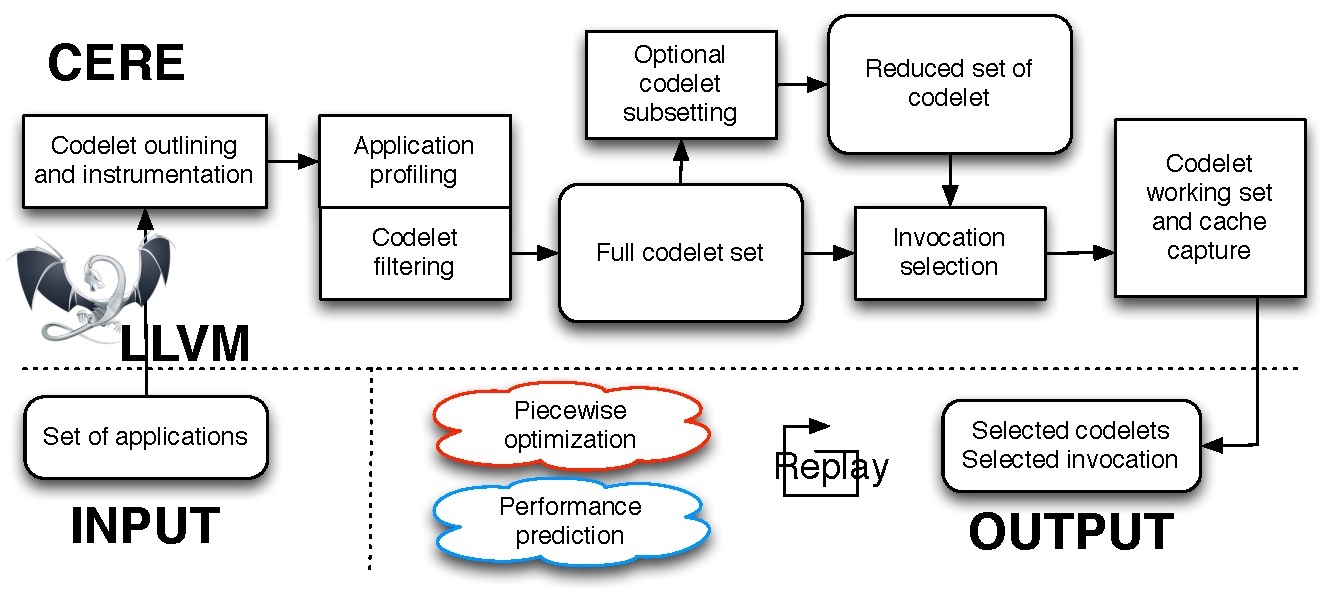
\includegraphics[width=0.85\linewidth]{cere_fonction.pdf}
\caption{\label{CERE_schema}Functional scheme of CERE (LLVM logo courtesy of Apple Inc.)}
\end{center}
\end{figure}

\newpage

\begin{multicols}{2}


CERE captures the memory context at a page-granularity level, which is lighter than a full dump and then faster to replace in memory when replaying inside a simulator. The memory capture allows to restore the codelet working set and cache-state before it is replayed. 


% PABLO: je ne comprends pas cette phrase. Peux tu clarifier stp ?
%This step should not be avoided when tuning microarchitecture parameters such as cache size or cache line size, as the warm-up could be slower but the other executions much faster.


\subsection{On the simulators}
\subsubsection*{The gem5 simulator}
The gem5 simulator is a cycle-accurate simulator. Its accuracy has been demonstrated on ARM simulation on both in-order and out-of-order processor, comparing real and simulated Cortex-A8 and Cortex-A9\cite{DBLP:conf/samos/EndoCC14}. These comparisons reveal an average absolute error of only 7\%.

Replaying SPLASH benchmark on gem5 shows an error on the execution time from 1.39\% to 17.94\%, explained by an inaccurate simulation of the DDR memory. Nevertheless, the gem5 simulator now handles different memory types, including modern DDR3, DDR4 and GDDR5, which should be more accurate than the tested DDR memory used in SPLASH tests\cite{DBLP:conf/recosoc/ButkoGOS12}.


\subsubsection*{The McPAT simulator}
McPAT is the first integrated power, area, and timing simulator. It can emulate both multicore and manycore systems with various technology, including in-order and out-of-order cores, caches, network chips, and several manufacturing processes. It can be used with several simulators thanks to its XML-interface (detailed in figure \ref{McPAT_schema}). McPAT computes both static (average power consumption of the CPU) and dynamic power consumption (peak power used when executing a specific task). We use dynamic power consumption in this paper, as we aim at finding the codelet with the highest performance/power ratio.
McPAT can also compute the die size of a simulated CPU, but this functionality has not been used in this paper.


In previous studies, McPAT accuracy has been validated against four real CPUs\cite{McPAT} and shows a relative error from $10.84\%$ to $22,61\%$. The simulated power is always under-evaluated, as some components present in the CPU are sometimes not taken into account. Similarly, the computed die size differs up to $27.3\%$ from the real processor.



\section{Simulation framework}
\label{sim}

\subsection{The gem5 simulator}

The gem5 simulator can be run in two different modes: syscall emulation (SE) and fullsystem mode (FS). The Syscall emulation mode simulates only the behaviour of the CPU inside a Linux operating system, and therefore cannot efficiently simulate multi-threaded application, as no scheduler has been implemented. Besides, SE mode requires a static linkage of all the application libraries.

On the contrary, the FullSystem (FS) mode emulates a full CPU; as the OS is emulated, the simulation is really slow (about fifteen minutes to boot Linux on an x86 AtomicSimpleCPU). Nevertheless, FS mode is more accurate and more flexible.

\end{multicols}
\begin{figure}[ht]
\begin{center}
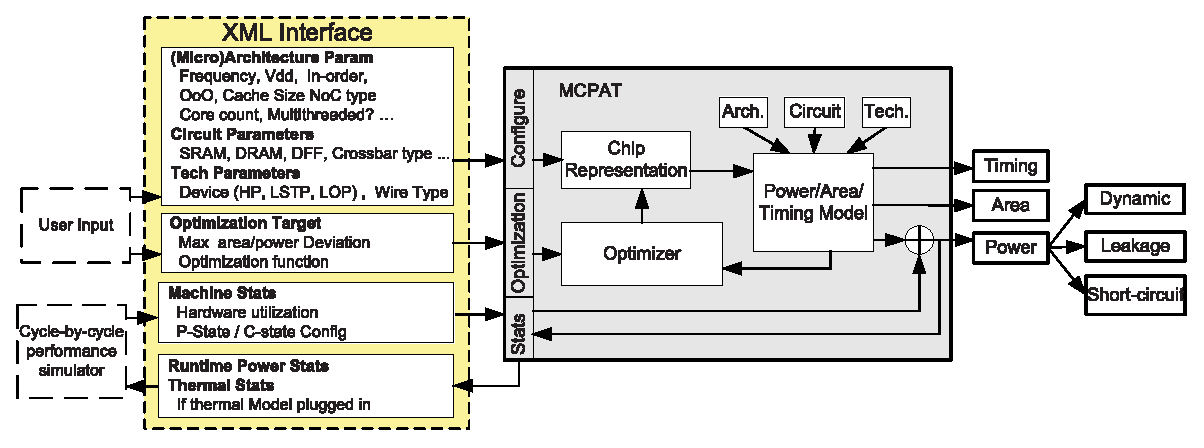
\includegraphics[width=0.9\linewidth]{McPAT_diag.eps}
\caption{\label{McPAT_schema}Functional scheme of McPAT}
\end{center}
\end{figure}

\newpage

\begin{multicols}{2}
Indeed, FS mode can handle dynamic libraries, assuming that they are well installed in the virtual disk image. 
Moreover, gem5 features a checkpoint functionality which avoids booting again when the CPU is changed.


\begin{Figure}
\centering
%%CHANGER LA LEGENDE "second"
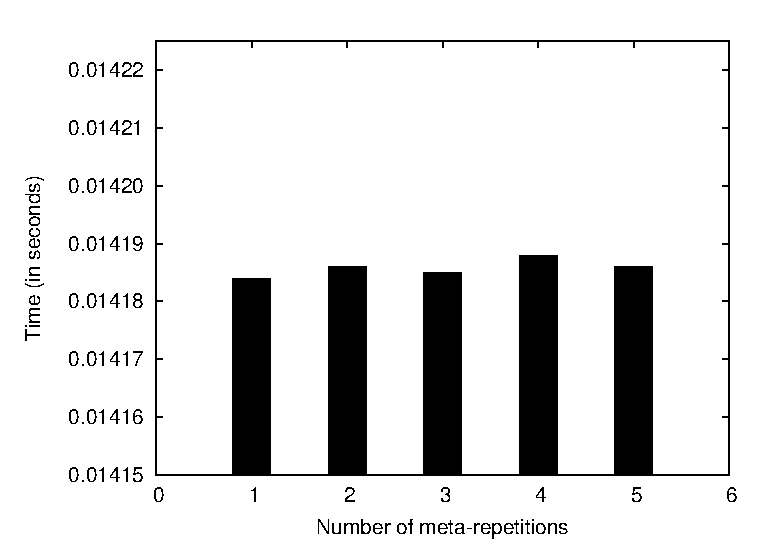
\includegraphics[width=\linewidth]{vari_se.eps}
\captionof{figure}{\label{vari_se}Variations of the codelet loop execution time on NAS IS class W benchmark using the i5-3550 configuration without turbo, with four CPUs.}
\end{Figure}

\subsubsection{Syscall emulation mode}
Gem5 required two code patches before CERE sequential codelets could be run in SE mode. First, the \textit{getdents} syscall has been implemented, which is called inside the \textit{readdir} function, used in the codelet memory mapping function.
The second change concern a bug occurring when reading EOF with the syscall \textit{read} while providing an invalid pointer: according to POSIX specifications it should work and write nothing, but caused a page fault in gem5. Both patches were submitted to the gem5 community.


In order to statically compile codelets with CERE\footnote{CERE version 0.2 was used in this paper.}, the argument \textit{-static} must be provided at the link time. Noting that this could provoked some relocation error when specifying the entry point of the program: offset 0x60000000 (used as default start point in CERE) is used to place the standard C library in sequential NAS IS. Experimentally, offset 0x40000000 did not cause any trouble when compiling sequential codelets. This issue has been fixed in the last version of CERE.

%Pablo: Pour info, j'ai implémenté le mode -static en suivant ton HOWTO et résolu le problème de l'offset. On n'a plus besoin du tout de préciser un relocation offset.

OpenMP parallel codelets cannot be run on SE mode due to the lack of real pthread implementation in the SE susbsystem. Indeed, statically linking with \textit{libiomp.a} results in a forced exit because of the missing pthread management syscalls.

\medskip
With these changes, and assuming that all the syscalls have been implemented inside the gem5 simulator, any sequential codelet should work in SE mode. Given that there is no scheduler in gem5 SE mode, and given that there is no proper implementation of pthread implementation in SE mode\footnote{M5thread has not been tested due the lack of scheduler and the miss of important syscall implementations in SE mode.}, parallel codelets cannot be realistically replayed on SE mode.


\medskip
Using the region \_\_cere\_\_is\_ranked\_475 with five meta-repetitions (six total runs of the loop, as one is used to warm the cache up), we observed 4x speedup, comparing to running the full benchmark\footnote{Class W inputs were used for all the results.}.

\end{multicols}


\begin{figure}[ht]
\begin{center}

\begin{tabular}{| l | c | c | c | c | c | c |}
\hline 
& & & \multicolumn{2}{c|}{L2} &\\
Name & Frequency\footnote{Non-turbo - Turbo frequency when turbo techology is implemented} & L1D and L1I associativity\footnote{The L1D and L1I size is always 32 kB.} & Size & Assoc. & L3 \\
\hline

Cortex-A15 & 1 GHz & 2 & 1 MB & 16 & No \\

i5-3550 & 3,3-3,7 GHz & 8 & $4 \times 256$ kB & 8 & Yes\footnote{The size of the L3 cache is set to 8MB and its associativity to 16-way due to gem5 limitations, it should be 6MB and 12-way.}\\

i5-3337U & 1,8-2,7\footnote{Only the non-turbo frequency has been simulated} GHz & 8\footnote{It should be 6 MB.} & $4 \times 256$ kB & 16 & Yes\footnote{It should be 3 MB.}\\

Q9100 & 2,26 GHz & 8 & 8 MB\footnote{It should be 6 MB and 12-way.} & 16 & No\\



\hline

\end{tabular}
\caption{\label{cpu_setup}Parameters used for CPU simulations.}
\end{center}
\end{figure}
\begin{multicols}{2}

All the data analysis is done on the median of these five meta-repetitions, but as the fluctuation is at most 0,03\% (figure \ref{vari_se})\footnote{This is due to the deterministic routine of the codelet, as the region \_\_cere\_\_is\_ranked\_475 is verifying that a give array is well-sorted. Such tight results were harder to get on non-deterministic or multithreaded code, see section \ref{FS_mode}.}, we can imagine running a codelet with only two or three meta-repetitions without significant bias.

\subsubsection{Fullsystem mode}
\label{FS_mode}
To run codelets in FS mode, only a few changes have been done: a manually prepared recent image based on Ubuntu-core 14.04 was used instead of the standard Ubuntu 7.04 image available on gem5 site. The kernel used is version 3.2.40 with default gem5 configuration.


To run OpenMP applications, just putting the \textit{libiomp5.so} and \textit{libomp.so} in \textit{/usr/lib}\footnote{Taken from linux mint MATE 17.3 64 bits} works. Therefore setting KMP\_affinity to \textbf{scatter}, which should assign each thread to a different core if available, results in a segmentation fault when starting the codelet. As a consequence, codelets on small inputs shows inexploitable behaviour (figure \ref{freqmine_nogood}) on four cores.
%CHANGE THE FIGUUURRRRRREEEE "seconds" sans "e" !!!
 Moreover, gem5 seems to hang when simulating more than one x86 CPU in FS mode, that is why all the applications (including multicore's one) were run using a one-core configuration.


\subsubsection{Chosen codelets}
We chose three codelets to efficiently reproduce different usages:
\begin{itemize}
\item NAS IS sequential: region \_\_cere\_\_is\_ranked\_475 which check whether the computed array is sorted or not.
\item PARSEC\footnote{Version 3.0-beta-20150206} x264: region \\ \_\_cere\_\_encoder\_analyse\_block\_residual\_write- \_cabac\_745 used in the CABAC encoding of the video\footnote{This codelet reveals to be unmeasurable, see \ref{results}}.
\item PARSEC blackscholes: region \\ \_\_cere\_\_blackscholes\_m4\_\_Z9bs\_threadPv\_first, an OpenMP region calculating the option value based on the Black \& Scholes's equation.
\item PARSEC freqmine: region\\ \_\_cere\_\_tree8scan1\_DBEP4Data\_first which generates a hash from the tree dataset.
\end{itemize}

\subsection{Simulation models}
\subsubsection{Hardware configuration}
The chosen configurations are detailed in figure \ref{cpu_setup}. All systems are set with 8 GB of 1600 MHz DDR3, the cacheline size is always kept at 64 B, and all CPUs are quad-core without hyper-threading.


McPAT simulates all the CPUs with a 44nm manufacturing process, to observe the impact on the power consumption of the architectural tuning only. The power consumption data correspond to the \textit{dynamic power} output of McPAT.

\begin{Figure}
\centering
\bigskip
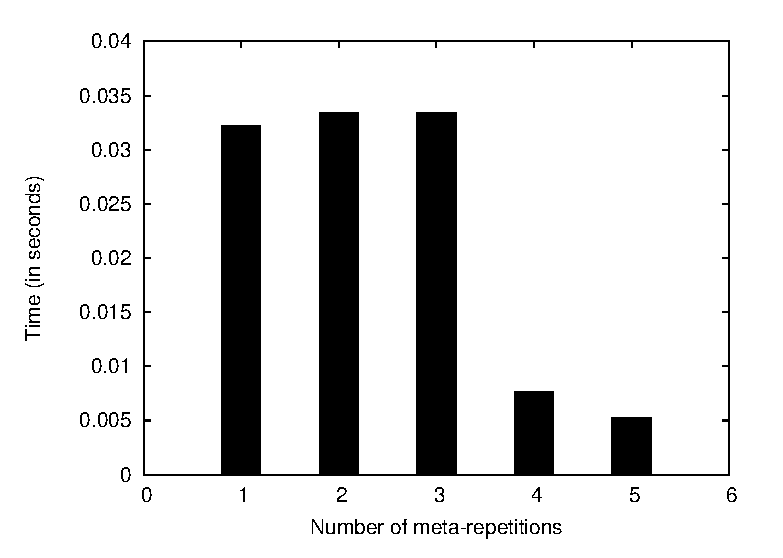
\includegraphics[width=\linewidth]{nogood.eps}
\captionof{figure}{\label{freqmine_nogood}Variations of the codelet loop execution time on PARSEC Freqmine benchmark using the Cortex-A15 configuration with four AtomicSimpleCPU and simtest input.}
\end{Figure}

\section{Results}
\label{results}
The power consumption of each CPU is calculated roughly using gem5 output file by the McPAT software: such value should not be taken absolutely but relatively to other CPU simulated. A power consumption of 10W is indeed too small for an one-core X86 desktop CPU running a benchmark. 

One have to keep in mind that the CPUs use only using a generic single-core x86 model, without hyper-threading or other recent technological improvements (pipeline aside). The absolute measures are therefore quite irrealistic. Nevertheless, the ratio between performance points provide interesting feedback to evaluate the fitness of a codelet to a given architecture.

\newpage %avoid warning
Unfortunately, X264 codelet execution is too fast to be measured with gem5 (only 0,0000001 or 0,0000002 seconds are calculated), so this codelet will only be analysed for its power consumption. 

% PABLO: je pense que même les mesures energétiques doivent être faussées par le temps d'exécution très court...
% Malheureusement en l'état les résultats x264 me semblent inexploitables. Mais ça arrive :-)


\subsection{Individual codelet results}

\subsubsection{IS: A serial applications}
IS codelet results are unsurprising and match quite well what one would expect when ranking the tested CPUs (see figure \ref{IS}): the most recent CPU, the i5-3550, is the fastest, either with or without boost. Boost only gives a small performance improvement. The Q9100 consumes less power, but is also less powerful. The lowest performance is given by the i5-3337U, a mobile processor, and the Cortex A-15.

As seen in figure \ref{IS_instr}, the instructions used are mostly integer one ($60,9\%$), following by load instructions ($30,4\%$), and store ($8,7\%$) instructions. IS does not use floating instructions at all, which explains the unsurprising linear performance variation of each CPU according to frequency: all of them use the same pipeline and integer compute units.
\begin{Figure}
\centering
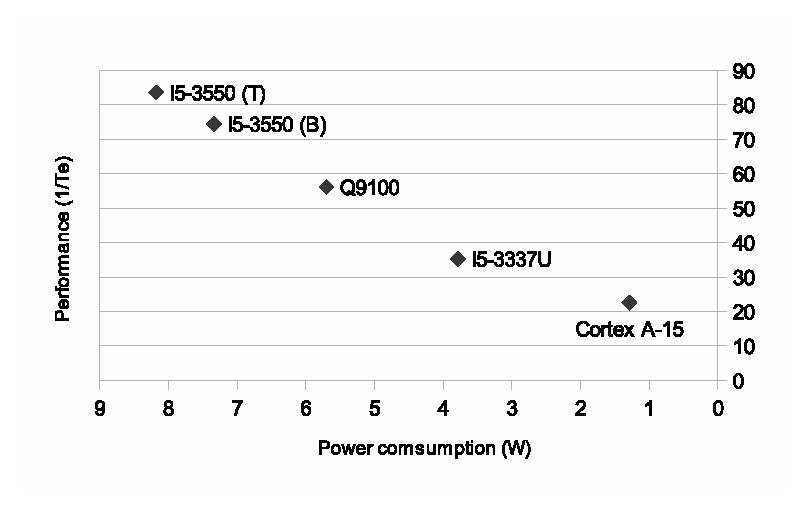
\includegraphics[width=\linewidth]{IS.eps}
\captionof{figure}{\label{IS}Power-Performance graph for the IS codelet.}
\end{Figure}

\begin{Figure}
\centering
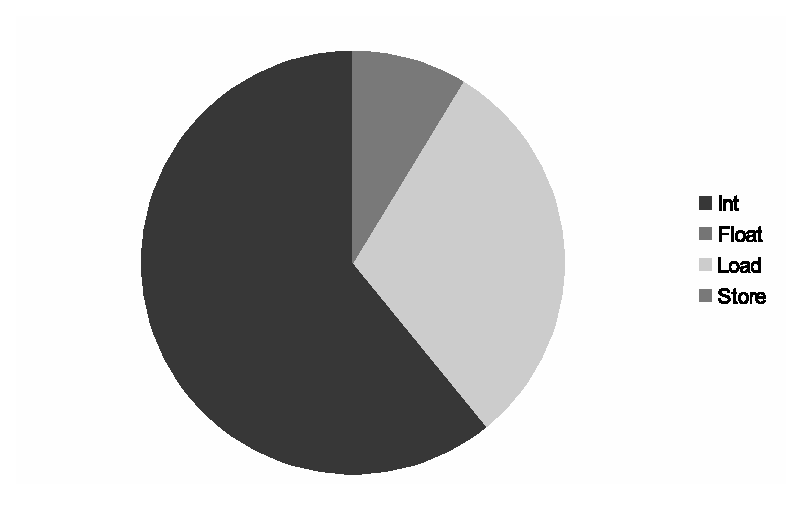
\includegraphics[width=\linewidth]{IS_instr.eps}
\captionof{figure}{\label{IS_instr}Repartition of the instructions during the execution of the IS codelet.}
\end{Figure}

\subsubsection{Parallel applications}
This parallel applications are run on a one-core configuration: these results are only bound to show the single-core performance-consumption differences, and not the manycore scaling. In future work, such measures could be replicated on ARM systems thanks to \ref{ARM_sim}.

\paragraph{Freqmine\\}
Freqmine was tested with a small data input that fits fully in cache. The Q9100 L2 cache is faster than the i5-3350 L3 cache, so the former is slightly faster than the latter at stock frequency on this benchmark - and consumes the same power (figure \ref{Freq}). With the turbo enabled, the i5-3550 stays first. Then follows the mobile i5-3337U, and finally the Cortex-A15

On the instruction repartition (figure \ref{Freq_instr}), freqmine is quite similar to IS: $56,5\%$ of integer instructions, $31\%$ of loading ones and $12,5\%$ of storing ones. As IS, freqmine does not use floating point units.

\begin{Figure}
\centering
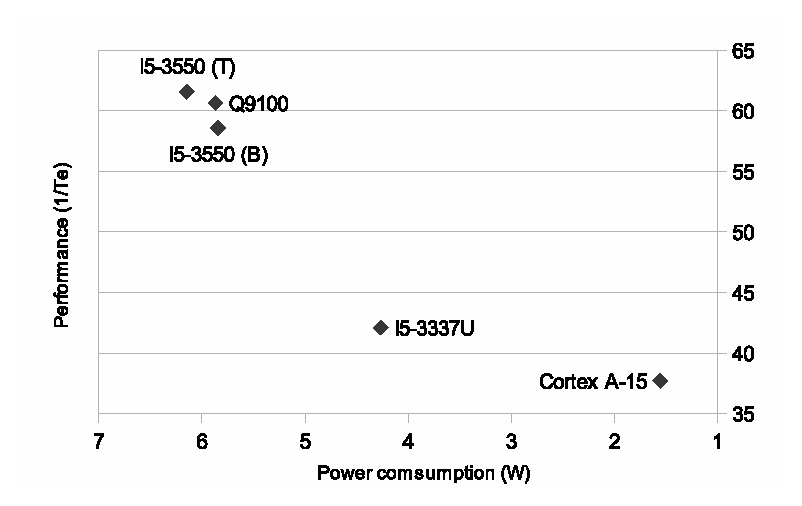
\includegraphics[width=\linewidth]{Freqmine.eps}
\captionof{figure}{\label{Freq}Power-Performance graph for the Freqmine codelet.}
\end{Figure}

\begin{Figure}
\centering
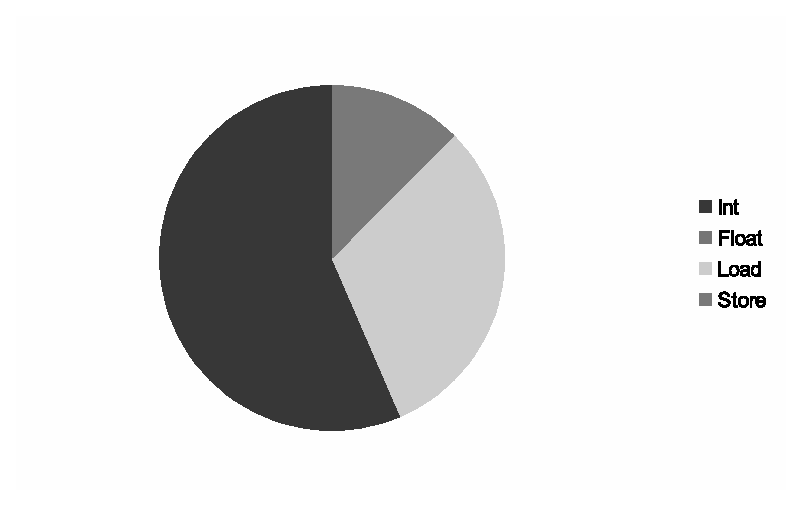
\includegraphics[width=\linewidth]{Freqmine_instr.eps}
\captionof{figure}{\label{Freq_instr}Distribution of the instructions during the execution of the Freqmine codelet.}
\end{Figure}


\paragraph{Blackscholes\\}
\label{Blackscholes}
Contrary to the other codelets, blackscholes uses floating operations. This application uses still mostly integer instructions ($56,7\%$), then floating operations ($23,8\%$), then $13,8\%$ of loading instructions, and finally $5,8\%$ of storing ones.


Here too, the CPUs follow the same performance ranking as for IS codelet: the i5-3550 first, then the Q9100, then the i5-3337U, ended by the Cortex-A15


\begin{Figure}
\centering
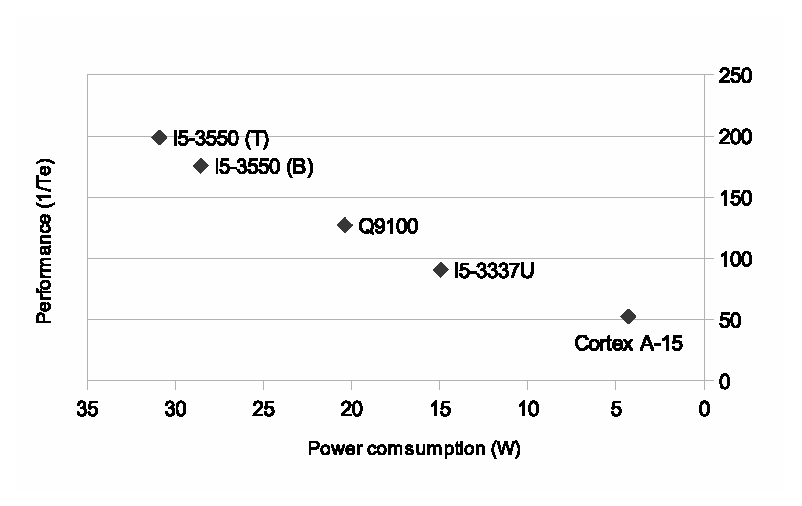
\includegraphics[width=\linewidth]{Blackscholes.eps}
\captionof{figure}{\label{Blasch}Power-Performance graph for the Blackscholes codelet.}
\end{Figure}

\begin{Figure}
\centering
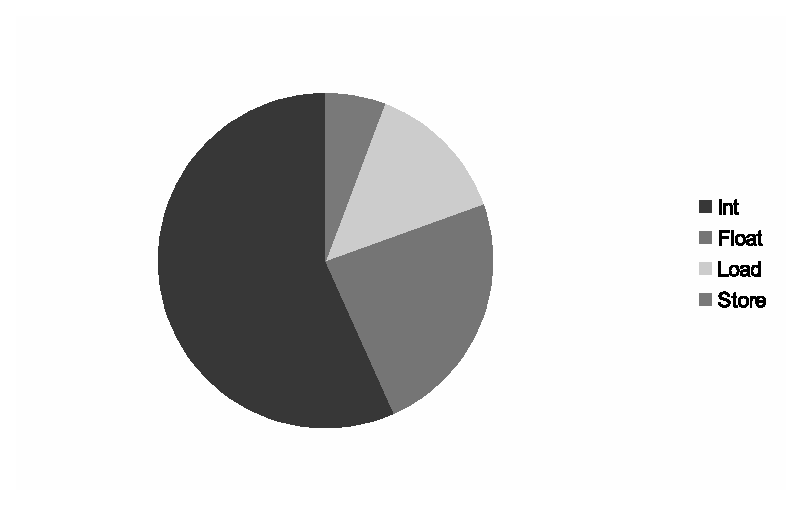
\includegraphics[width=\linewidth]{Blackscholes_instr.eps}
\captionof{figure}{\label{Blasch_instr}Distribution of the instructions during the execution of the Blackscholes codelet.}
\end{Figure}

\subsection{Performance}
The performance of all tested CPU on IS, blackscholes and freqmine is represented figure \ref{Perf}.

\begin{Figure}
\centering
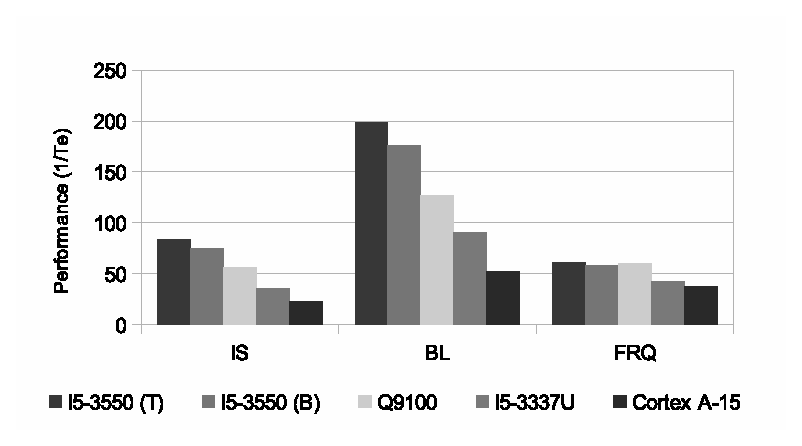
\includegraphics[width=\linewidth]{Performance.eps}
\captionof{figure}{\label{Perf}Performance of all tested CPUs on differents codelets.}
\end{Figure}


IS and freqmine have a close execution time (figure \ref{Perf}), even if freqmine codelet was extracted running the simtest input. Besides, the relative gap between the Cortex-A15 and the high-end X86 CPUs is particularly vivid on IS and blackscholes codelets. On freqmine, the performance difference becomes really smaller. Once more, this is due to the simtest input, smaller, which fits in the 1MB L2 cache of the cortex-A15.


\subsection{Power consumption}
When the power consumption is on the $x$ axis, the former is graduated backward to keep a \textit{higher-is-better} index.


\begin{Figure}
\centering
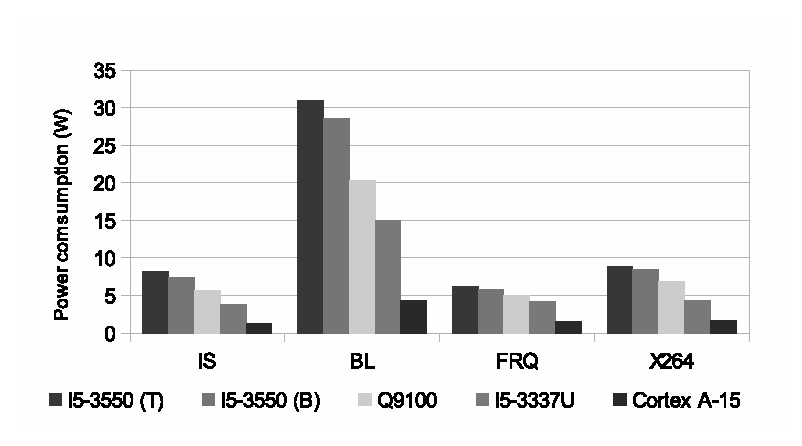
\includegraphics[width=\linewidth]{Power_consumption.eps}
\captionof{figure}{\label{Pow}Power consumption for each CPU.}
\end{Figure}

The blackscholes codelets seems to consume more power than all the other codelets (figure \ref{Pow}). This is due to floating point operations, used significantly only in this codelet (see \ref{Blackscholes}).

Even if every simulation treats the Cortex A-15 as an X86 CPU, its power consumption is from $4,0$ to $7,2$ times smaller than the i5-3550 with turbo. This tends to show than the power consumption is mostly an architectural parameter and not a characteristic of the instruction set.


\subsection{Power/performance measurement}
\subsubsection{Definition of the power/performance index}
The performance of a CPU is measured by the execution time of the selected codelet. To keep an higher-is-better index, only $1/t_e$ values are used (where $t_e$ is the execution time in seconds).
The power-consumption ratio is defined as 
\begin{equation}
I=\frac{1}{P.t_e}
\end{equation}
With $P$ the power consumption of the CPU on the benchmark in Watt.

A higher ratio means either better performance or less consumption, and so a better choice.

\bigskip

This ratio can also be seen as follow:\\
$C=k.P.T_e$ is the cost to run an application with:
\begin{itemize}
\item $k$ is the cost of power.
\item $P$ and $T_e$ the same notation as before.
\end{itemize}


So $I=\frac{k}{k.P.T_e}$ is only the inverse of the normalized price paid to run the benchmark. We keep an higher-is-better index, as we aims at minimizing the operating cost.




\subsubsection{Results on the test panel}


The power/performance ratio for each codelet is compared on figure \ref{Ratio}. The ARM Cortex-A15 is by far the best option for every codelet, if one wants to minimise the power/performance ratio.

\begin{Figure}
\centering
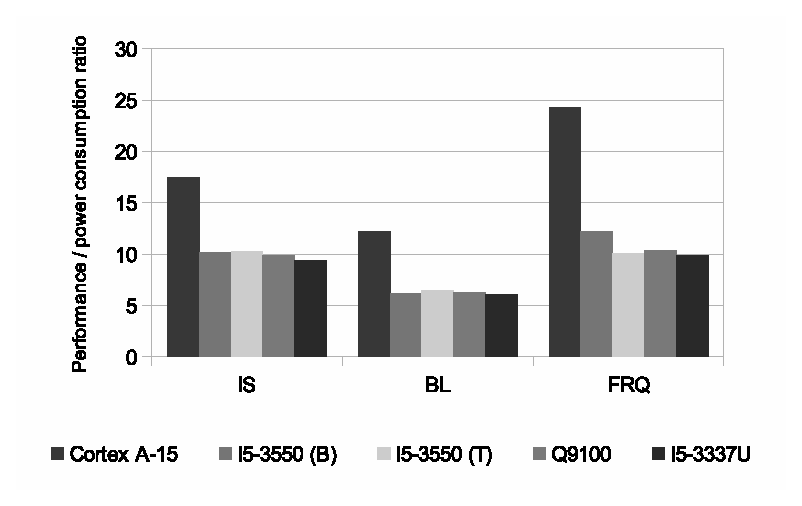
\includegraphics[width=\linewidth]{Ratio.eps}
\captionof{figure}{\label{Ratio}Performance-Power consumption ratio for each codelets.}
\end{Figure}

This CPU aside, the classic X86 ones do not show some great relative differences. Therefore, blackscholes seems to limit the advance of the Cortex-A15: the small associativity of L1D and L1I probably limits it on floating operations.


\subsection{Advantages}
The use of codelets gives a powerful tool to fine-tune the architecture and codelet co-design. Because of CERE limitations, only codelets replay \textit{for} loops or \textit{omp parallel for} loops are supported, but this is much lighter than running the full application. Moreover, codelets can improve individually each region of an application, which enables per-region mapping when running on a big.LITTLE system, or any heterogeneus computer server.

The gem5 simulator is a precise tool to reproduce the behaviour of a specific machine on a general computer. As the simulation is quite slow, the use of codelets could be really useful in term of time and resources in the conception of heterogeneous servers. As CERE operates as an IR-level, the operation does not need any additional work on the source code, and can be run in C, C++ or Fortran programs. Besides, the compilation of the codelets uses the power of the host machine and not the simulated one, which is really useful in term of compute time: the emulated system is used only when it is truly needed.

\subsection{Inconvenients}
Gem5 is a simulator, and therefore cannot be entirely trusted. CERE too cannot exactly replay a whole execution of an application ; and the measures output by McPAT are only an estimation of the effective power consumption of the CPUs: that's why the results could not fit exactly to the real-life experiments. Nevertheless, these simulations are bound to give an overview of the gains that could be archived by improving a specific part of a CPU, not to give absolute results.

The gem5 simulator has not been validated yet on x86 accuracy, and could be quite biased, as it emulates a generic x86 processor, whereas state of the art CPUs are even more complex.

Besides, the power consumption is not exactly the right parameter to adapt, as one prefers usually a fast machine consuming a bit more than a really slow one.

Moreover, the manufacturing costs has never been reckon with in this paper, whereas architectural tuning needs a material support for further implementations. 


\section{Conclusion}
\label{ccl}
This paper presents a novel approach on a hardware-to-software adaptation using codelets to speed up gem5 simulations. 

The use of codelets is faster and nearly as efficient as regular benchmarks; and the combine use of gem5 along with McPAT offers a powerful and flexible tool to simulate any architecture modification on compute units.

Our primary results validate the fact that ARM architecture consumes really less power than X86 standard one, unsurprisingly. But its power-performance ratio is up to 7 times better than a regular i5. On the hardware side, the cache size plays an important role in the performance, so one can imagine that some specific architecture could be developed, fitting the cache size (or type) to the data used for example.

Even if only four CPUs are simulated, this results encourage to wisely choose the right architecture when selecting the hardware. A conjoint development of future architecture, based on their efficiency for a specific use only, would be a great step forward in the conception of new architectures and lead to lower power consumption. 

\newpage

\bibliographystyle{plain}
\bibliography{report}


\newpage
\section{Annexe}
\subsection{ARM Simulation}
\label{ARM_sim}
As multicore benchmarks seem to hang on X86 simulation, some work has been done to adapt the codelet on ARM simulation.
The multicore simulation works with linaro-minimal.

As capturing on ARM required an ARM machine, a few cross-compile instructions has been added in CERE. Capturing on gem5 may indeed take several days, and require moreover an ARM version of CERE pre-installed on the virtual machine, which was not ready at the time of this work. The goal is then to use an x86 memory dump and replay it on ARM systems. The following changes were made in CERE:
\begin{itemize}
\item Changed objdump to aarch64-linux-gnueabi-objdump.
\item Added clang cross-compile option.
\end{itemize}

After those changes, the compilation ran successfully, but the execution outputs \textit{"Killed"}, even before the main() starts.


We found that the aarch64 architecture limits the application space to the address 0x00000000\_00000000 to 0x0000ffff\_ffffffff\cite{aarch64-mmu}.
%PUT A PICTURE !!!!!
 But the stack is placed on x86 linux at address 0x07fda3c7\_b0000000 so the kernel kills the application as soon as the X86 stack region is reserved.
To avoid this issue, the stack has manually been moved to address 0x000003c7\_b0000000.

NAS IS (codelet \_\_cere\_\_is\_ranked\_475) has been successfully replayed on a juno board (linaro-image-minimal-genericarmv8 system) using this trick. Nevertheless, further adaptations have to be done in order to safely convert x86 dumps to ARM dumps\footnote{Especially on pointers of stack address which need to be updated to the new stack position at the codelet compilation.}.


\subsection{About the UVSQ laboratory}
TODO

\subsection{Gem5 patches}
TODO

\end{multicols}

\end{document}
